%\documentclass[12pt,spanish,fleqn,openany,letterpaper,pagesize]{scrbook}

\usepackage[utf8]{inputenc}
\usepackage[spanish]{babel}
\usepackage{fancyhdr}
\usepackage{epsfig}
\usepackage{epic}
\usepackage{eepic}
\usepackage{amsmath}
\usepackage{threeparttable}
\usepackage{amscd}
\usepackage{here}
\usepackage{graphicx}
\usepackage{lscape}
\usepackage{tabularx}
\usepackage{subfigure}
\usepackage{longtable}


\usepackage{rotating} %Para rotar texto, objetos y tablas seite. No se ve en DVI solo en PS. Seite 328 Hundebuch
                        %se usa junto con \rotate, \sidewidestable ....


\renewcommand{\theequation}{\thechapter-\arabic{equation}}
\renewcommand{\thefigure}{\textbf{\thechapter-\arabic{figure}}}
\renewcommand{\thetable}{\textbf{\thechapter-\arabic{table}}}


\pagestyle{fancyplain}%\addtolength{\headwidth}{\marginparwidth}
\textheight22.5cm \topmargin0cm \textwidth16.5cm
\oddsidemargin0.5cm \evensidemargin-0.5cm%
\renewcommand{\chaptermark}[1]{\markboth{\thechapter\; #1}{}}
\renewcommand{\sectionmark}[1]{\markright{\thesection\; #1}}
\lhead[\fancyplain{}{\thepage}]{\fancyplain{}{\rightmark}}
\rhead[\fancyplain{}{\leftmark}]{\fancyplain{}{\thepage}}
\fancyfoot{}
\thispagestyle{fancy}%


\addtolength{\headwidth}{0cm}
\unitlength1mm %Define la unidad LE para Figuras
\mathindent0cm %Define la distancia de las formulas al texto,  fleqn las descentra
\marginparwidth0cm
\parindent0cm %Define la distancia de la primera linea de un parrafo a la margen

%Para tablas,  redefine el backschlash en tablas donde se define la posici\'{o}n del texto en las
%casillas (con \centering \raggedright o \raggedleft)
\newcommand{\PreserveBackslash}[1]{\let\temp=\\#1\let\\=\temp}
\let\PBS=\PreserveBackslash

%Espacio entre lineas
\renewcommand{\baselinestretch}{1.1}

%Neuer Befehl f\"{u}r die Tabelle Eigenschaften der Aktivkohlen
\newcommand{\arr}[1]{\raisebox{1.5ex}[0cm][0cm]{#1}}

%Neue Kommandos
\usepackage{Befehle}


%Trennungsliste
\hyphenation {Reaktor-ab-me-ssun-gen Gas-zu-sa-mmen-set-zung
Raum-gesch-win-dig-keit Durch-fluss Stick-stoff-gemisch
Ad-sorp-tions-tem-pe-ra-tur Klein-schmidt
Kohlen-stoff-Mole-kular-siebe Py-rolysat-aus-beu-te
Trans-port-vor-gan-ge}

%\begin{document}

\justifying
\chapter{Modelando la población del vector de Dengue utilizando datos de sensado
        remoto y aprendizaje automático}

  \par Como mencionamos en capitulos anteriores, en un contexto interinstitutional entre
    la Comisión Nacional de Actividades Espaciales (CONAE) y el ministerio de salud
    de Argentina, se han desarrollado iniciativas orientadas a modelar la evolución temporal de
    las poblaciones de mosquitos usando variables ambientales obtenidas de
    sensores remotos. Estos trabajos utilizaron series de algunos años y fueron
    basadas en un pequeño número de variables satelitales \cite{ndwi_erffectiveness, modis_data}.
    En un esfuerzo para mejorar esto, construyeron modelos
    de series temporales de cuatro años, basados en una gran cantidad de variables
    de varios sensores\cite{temporal_modeling}.
    Aún así, todos estos trabajos asumieron modelos lineales multivariados.

  \par Como parte del trabajo presentado en este capítulo se desarrolló un
    sistema
    para la generación y evaluación de modelos basados en aprendizaje automático.
    Ésto brinda a la comunidad de profesionales que
    aborda las problemáticas relacionadas con la epidemiología, una herramienta
    de alto valor dado que les permite realizar,
    modelos de evolución de población de mosquitos.

  \par A su vez, este trabajo representa una
    mejora en la capacidad de modelado con respecto a los esfuerzos previos ya
    mencionados. En éste se comparan distintos algoritmos de
    aprendizaje automático: Support Vector Machines (SVM),
    Redes Neuronales Artificiales (ANN), K-vecinos más cercanos (KNN) y un tipo
    de árbol de decisión orientado a regresión.
    Se suman a la comparación dos modelos de regresión lineal.
    Con ésto, se
    obtiene una metodología operacional que podría contribuir al sistema de riesgo
    de Dengue actualmente en operación \cite{porcasi_operative, analisis_cordoba}.

  \par Adicionalmente, se explora, en contraste con los trabajos previos mencionados,
    la habilidad de modelado y predicción de oviposición con algoritmos de aprendizaje
    automático \textit{off-the-shelf}, i.e. algoritmos de software libre, ya
    implementados, sin mayores desarrollos sobre lo existente y con un ajuste de
    hiperparámetros minimo. De ésta manera se busca la asimilación de estas
    técnicas a toda la comunidad que se ocupa de problemas similares.

  \par Finalmente, resulta relevante mencionar que el trabajo
    realizado y descripto aquí ha dado lugar a la publicación
    \textit{Modeling Dengue Vector Population Using Remotely Sensed Data and
    Machine Learning} \cite{scavuzzo2018modeling} en la revista \textit{Acta Tropica}
    de \textit{Elsevier} (\url{https://www.journals.elsevier.com/acta-tropica}).

\section{Obtención, análisis y selección de datos a utilizar}

\subsection{Datos de estudio y Datos de Campo}
  \begin{figure}[hbt]
  \centering%
  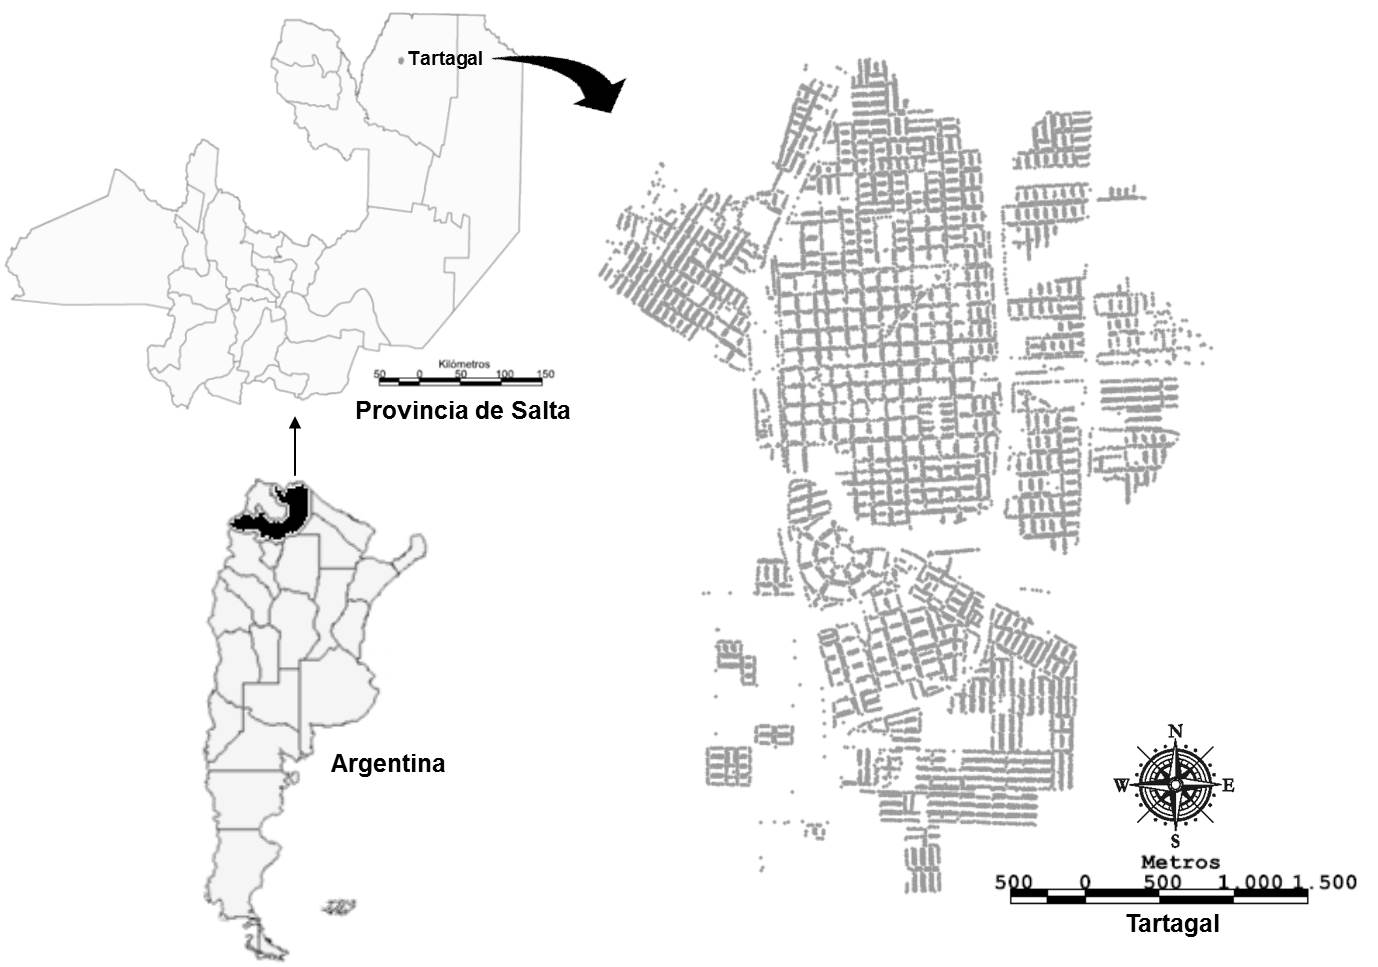
\includegraphics[width=0.6\textwidth]{images/tartagal}%
  \caption{Área de Estudio}\label{fig:tartagal}
  \end{figure}

  \par El estudio presentado fue desarrollado en la ciudad de Tartagal
    (con 79.900 habitantes) en el noroeste de Argentina
    (\ang{22;32;}~S, \ang{63;49;}~O, \SI{450}{\meter} sobre el nivel del mar),
    en la provincia de Salta. El sitio está entre 50 y 100 kms de la frontera
    entre Argentina y Bolivia, como se puede apreciar en la Figura \ref{fig:tartagal}.

  \par Este lugar tiene una temperatura media anual de unos \SI{23}{\degreeCelsius}
    (máximo promedio de verano de \SI{39}{\degreeCelsius} y minimo promedio en
    invieron de \SI{9}{\degreeCelsius}). Tiene una precipitación anual de
    \SI{1100}{\milli\meter}, con una estación seca (Junio a Octubre).
    Tartagal, como muchas ciudades del noroeste argentino, tiene una diversidad
    cultural basada en la presencia de grupos étnicos autóctonos y población
    de inmigrantes sumada al movimiento de migración proveniente de Bolivia.
    Estas características conducen a un perfil peculiar de comportamiento
    cultural, social y economico.

  \par La población de vectores es medida monitoreando la actividad de oviposición.
    Para ello se utilizan ovitrampas colocadas en casas aleatoriamente seleccionadas
    en el área urbana de la ciudad. El período de monitoreo utilizado en este
    estudio fue de Agosto de 2012 hasta Julio de 2016 sobre 50 casas. Dos
    ovitrampas fueron colocadas en cada una: una dentro y otra fuera,
    en el patio trasero en un lugar con sombra y a nivel del suelo, siguiendo
    las instrucciones de la OMS \cite{peridomestic}. Las ovitrampas son contenedores
    de \SI{1000}{\centi\meter\cubed} de plástico negro con \SI{250}{\milli\liter}
    de agua sin ninguna infusión de atracción.
    En este estudio sólo utilizamos los datos de las ovitrampas externas dado
    que ellas tienen una mayor correlación con las variables ambientales
    derivadas de información satelital. Dichas ovitrampas son reemplazadas
    semanalmente y los huevos son contados en un laboratorio de acuerdo al
    \textit{Indice de Densidad de Huevos} \cite{indice_huevos}. Luego, la
    actividad de oviposición del \textit{Aedes Aegipty} es estimada por la suma
    de los huevos capturados en las trampas externas de la ciudad.



\subsection{De productos satelitales a variables ambientales: conjunto de datos para el modelado}

  \par Siguiendo la idea de construir modelos predictivos de la población de
    vectores basados en variables ambientales derivadas de satelites, pero con una
    perspectiva operacional basada en trabajos previos, se generaron representaciones
    de vegetación, humedad, temperatura y lluvia operacionalmente disponibles
    de \textbf{MODIS} y productos \textbf{TRMM/GPM}.

  \par Los índices de vegetación global proveen productos espaciales y
    temporales consistentes sobre la cobertura de la vegetación,
    propiedades del área foliar y el nivel de clorofila. Estos indices son
    derivados de la reflectancia atmosférica
    corregida en las bandas infrarroja media (MIR, por sus siglas en inglés) y
    cercana (NIR, por sus siglas en inglés).
    En este trabajo se utiliza el \textbf{NDVI} del producto satelital
    de MODIS, \textit{MOD13Q1}, (compuesto de 16 días) con una resolución espacial de
    \SI{250}{\meter}.
    Las condiciones de vegetación son incluidas junto con la temperatura,
    humedad y precipitación, las cuales son variables relevantes para la evolución de la
    población de mosquitos \cite{ndwi_erffectiveness, rs_invertebrate}.

  \par A su vez, se incluye el Indice de Agua de Diferencia Normalizada
    (\textbf{NDWI}), que está vinculado al contenido de agua líquida y humedad
    tanto en la vegetación como en estructuras sólidas.
    Es calculada a partir del mismo producto MODIS usando la definición de
    \textit{Gao} \cite{gao_ndwi} del NDWI desde las bandas provistas por
    el producto \textit{MOD13Q1}, correspondiente a la reflectancia de MIR y NIR:
    $NDWI =  (\rho_{NIR} - \rho_{MIR}) / (\rho_{NIR}  + \rho_{MIR} ) \times 10^4$.
    Los productos MODIS, en general, necesitan el factor $10^{4}$ para ser guardados,
    por eficiencia computacional, como números enteros.

  \par Por su parte, utilizamos la temperatura de la superficie
    terrestre (\textbf{LST}) de MODIS dado que es una aproximación de la
    temperatura ambiental \cite{infectious_diseases, surface_temp, temp_algorithm}.
    Para esto, se eligió el producto satelital \textit{MOD11A2}. Éste tiene una
    resolución espacial de \SI{1}{\kilo\meter} y es un promedio de valores de
    LST de cielo-abierto durante un periodo de 8 días. Este producto incluye
    LST de la noche y del día para así, de alguna manera, representar
    temperaturas mínimas y máximas \cite{lst_surface}.

  \par Finalmente, la precipitación local es obtenida de la
    \textit{Misión Tropical de Medida de Lluvia}
    (\textbf{TRMM}) \cite{trmm_mision}. Ésta es una misión conjunta entre la
    NASA y la Agencia Aeroespacial de Exploración de Japón lanzada en 1997
    para el estudio de las lluvias y así realizar investigaciones sobre el
    clima. Para detectar la lluvia, el satélite utiliza muchos instrumentos
    incluyendo radar, imágenes de microondas y sensores de rayos. TRMM, a pesar
    de que se quedó sin combustible en 2014, siguió transmitiendo datos hasta
    Junio del 2015.
    Luego de eso, otros productos basados en una nueva misión espacial llamada
    GPM (\url{https://earthdata.nasa.gov/trmm-to-gpm}), fueron publicados para
    asegurar la continuidad de estos trabajos.


  \par Dos áreas de \SI{85}{\hectare} fueron definidas alrededor de la ciudad
    y se calcularon los valores medios para todas las variables derivadas de
    satelite. Siguiendo el enfoque de
    \cite{models_predicting, dynamics_of_dengue, temporal_modeling},
    la primer área se encuentra ubicada dentro de la ciudad
    (Área Urbana) y la segunda abarca la vegetacion nativa que rodea la ciudad
    (Área Rural). Ésta elección fue tomada bajo la hipótesis de que seleccionar
    una zona fuera de la ciudad representaría bien las condiciones ambientales
    (NDWI, NDVI, LST). La misma idea fue utilizada en estudios previos muy
    relacionados. Como se explica en dichos trabajos previos, es esperable
    que estas observaciones y los índices de larvas
    estén estrechamente relacionadas. En ese sentido es que el área rural o
    externa fue seleccionada aleatoriamente de aquellas con vegetación suficientemente
    cercana a la ciudad, representando condiciones ambientales naturales.
    En este caso específico esta región rural es seleccionada en el
    noreste de la ciudad; tiene una altitud similar a la ciudad y mayormente
    bosque nativo. Se puede observar en la Figura \ref{fig:zones}.
    \begin{figure}[hbt]
    \centering%
    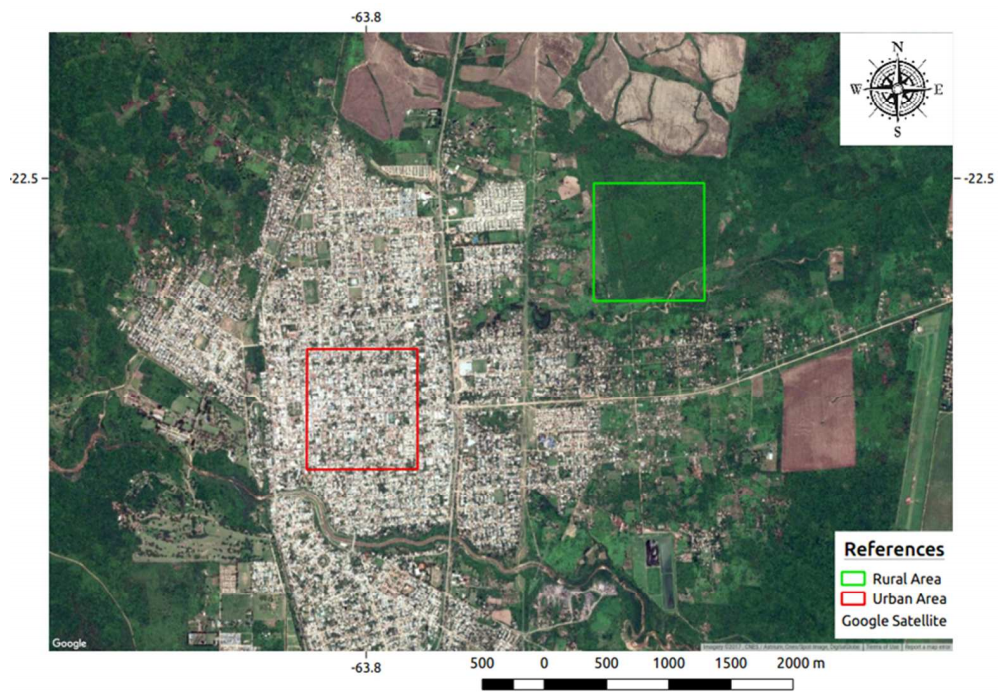
\includegraphics[width=0.6\textwidth]{images/zones}%
    \caption{Areas rural y urbana seleccionadas para extraer las variables ambientales}\label{fig:zones}
    \end{figure}


  \par El procedimiento de construir las series temporales a partir de variables
    provenientes del sensado remoto se describen en la Figura \ref{fig:sistema}.
    Las imágenes son obtenidas de la NASA (\url{http://e4ftl01.cr.usgs.gov}) e
    importadas en \textbf{GRASS 7.1}. Para cada una de las áreas anteriormente
    definidas se calcula la media de cada día. Cada uno de estos valores
    promedio y sus fechas son exportadas a una tabla en el software \textbf{R},
    donde es utilizada para construir las series temporales completas.
    Los datos son interpolados para obtener valores para cada uno de los
    días de muestra (un valor para cada semana epidemiológica) \cite{german_temporal}.
    \begin{figure}[hbt]
    \centering%
    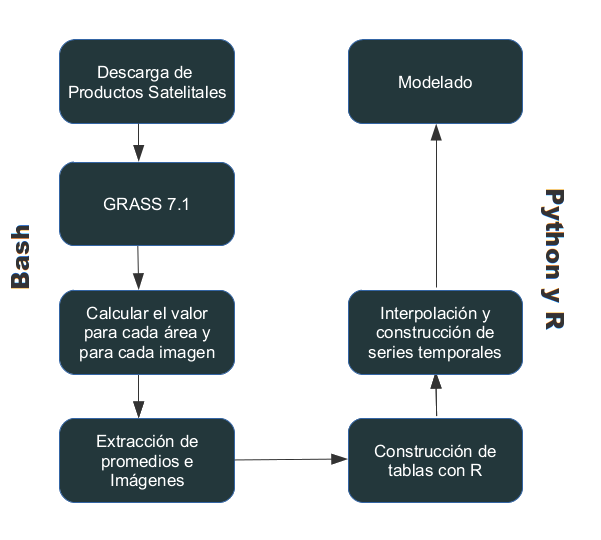
\includegraphics[width=0.6\textwidth]{images/sistema}%
    \caption{Sistema de procesamiento de productos satelitales}\label{fig:sistema}
    \end{figure}

  \par Todas las variables son consideradas con hasta tres semanas de
  \textit{lag}\footnote{Para un punto en el tiempo $t$, el valor de la variable
  $v_{1 lag_{1}}(t)$ es igual al valor de la variable $v_{1}(t-1)$ correspondiente
  al punto en el tiempo de una semana anterior.}
    teniendo en cuenta las series temporales originales, para representar las
    influencias asincrónicas, correspondientemente con uno, dos o tres
    lapsos de tiempo.

  \par El primer paso consistió en analizar las cuarenta variables ambientales
    y los huevos recolectados cada semana por medio de una matriz de correlación
    y los valores \textbf{p} que miden su significancia. Ésto llevó a descartar
    treinta y cinco variables. Se prefieren las variables con \textit{lag} dada
    su potencial habilidad de pronóstico \cite{german_temporal}. Las siguiente
    variables fueron seleccionadas: NDVI rural \textit{lag} 1,
    NDWI rural \textit{lag} 1, LST rural dia \textit{lag} 3,
    LST rural noche \textit{lag} 1 y TRMM \textit{lag} 3.
    Luego, todas las variables fueron normalizadas utilizando el
    \textbf{\textit{z-score}}\footnote{Técnica para normalizar datos en función de
    la media y desviación estándar muestrales}.

  \par La Figura \ref{fig:heatmap} presenta las variables ambientales junto
    con la oviposición en un mapa de calor (\textit{heatmap}). Este formato
    permite una visualización en la evolución temporal, de los
    patrones de correlación entre las variables y el efecto de \textit{lag}.

    \begin{figure}[hbt]
    \centering%
    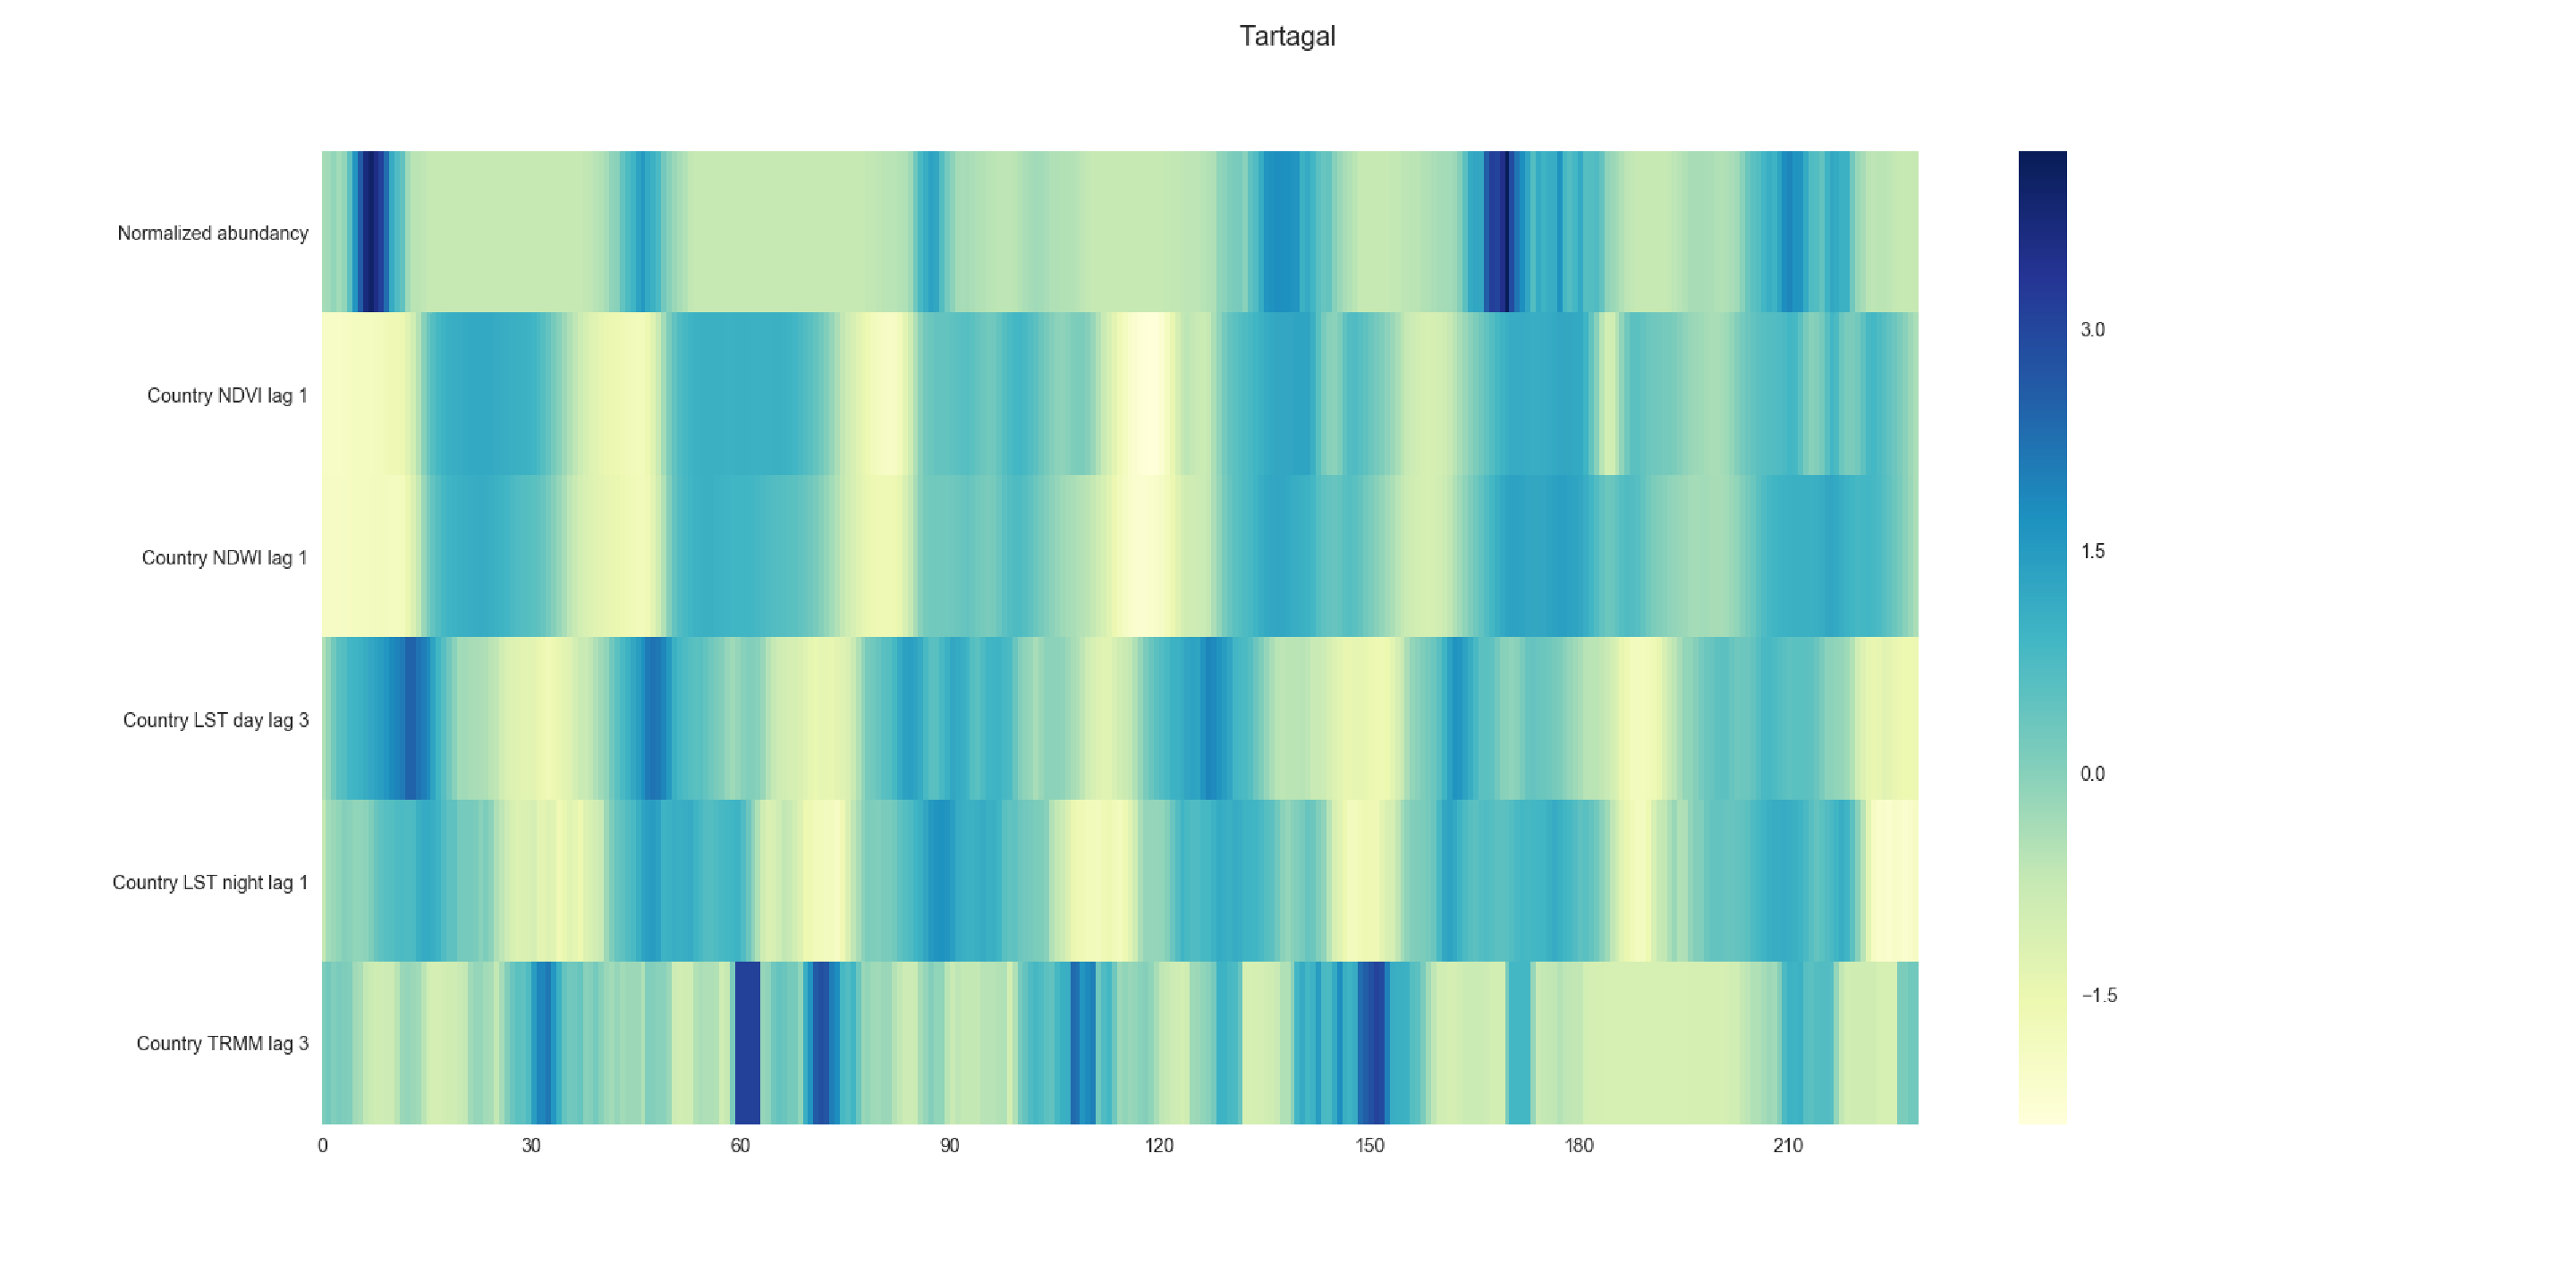
\includegraphics[width=1\textwidth]{images/heatmap}%
    \caption{Heatmap de valores del \textit{z-score} de variables ambientales}\label{fig:heatmap}
    \end{figure}



\section{Modelado}

  \par Con el conjunto de datos descripto en la sección anterior, se implementaron
    dos modelos lineales (tradicional y \textit{Ridge}) y cuatro modelos
    no-lineales (\textit{Support Vector Machine}, ANN Perceptron Multicapa,
    Árbol de Decisión, K-vecinos más cercanos) para modelar la oviposición
    para cada semana. Para todos los modelos se utilizó el mismo conjunto de
    5 variables ambientales como \textit{features}.

  \par En todos los casos se entrenaron los modelos con 80\% del conjunto de
    datos y se utilizó el 20\% restante de la serie temporal (alrededor de un año)
    como un conjunto independiente para validar la capacidad de predicción temporal
    de las herramientas (se usó el 20\% más "nuevo" del conjunto). Esta elección
    de porcentajes de división es la más utilizada en la literatura de ML \cite{ml_rainfall}.

  \par Se utilizó \textbf{Validación Cruzada}
    (\textit{Cross Validation}) \cite{cross_validation, ml_rainfall} con el
    objetivo de reducir la dependencia de los resultados en una selección particular
    del par de conjuntos de entrenamiento y validación. En particular, para
    evaluar los modelos, se utilizó un procedimiento de validación cruzada
    particular para problemas que involucran series temporales
    \url{http://scikit-learn.org/stable/modules/cross_validation.html}.
    Otras técnicas de validación cruzada como \textit{K-folds} no son
    adecuadas para los datos que se corresponden con series temporales, i.e,
    cuando el orden en el conjunto de datos es importante.

    \par A continuación se describirán las técnicas utilizadas para modelar
    el \textit{z-score} de la oviposición como una función variables ambientales
    extraidas de sensores remotos. Todos los modelos fueron implementados utilizando
    funciones de la librería \textbf{\textit{scikit-learn}}.

    \par La última, es una librería del lenguaje de programación Python, de libre
    acceso, para Aprendizaje Automático contruida sobre \textit{SciPy}\cite{scipy}.
    Es una herramienta sencilla y efectiva para minería y análisis de datos que
    proporciona un conjunto de utilidades que permiten una implementación
    completa de la solución de un problema de ML.
    Dado que está bajo licencia \textit{BSD}, esta librería puede ser utilizada
    tanto para uso personal como comercial.


    \subsection{Sistema de Modelado}

      \subsubsection{Requerimientos}
        \par Dado el objetivo de este trabajo, los requerimientos del mismo se
          basaron en la compatibilidad con lo publicado en el artículo ``\textit{An operative dengue risk stratification system in
argentina based on geospatial technology}" \cite{porcasi_operative}.
          Luego de un análisis del mismo, se concluyó que el sistema de
          modelado debe poseer las siguientes características:
          \begin{itemize}
            \item Facilidad de utilización para un usuario no especialista del área de
              Ciencias de la Computación.

            \item Poseer una herramienta de limpieza del conjunto de datos
              dado, para construir automáticamente los datos que luego
              utilizarán los distintos algoritmos.

            \item Versatilidad para su uso con otros conjuntos de datos sin necesidad
              de realizar mayores cambios en la arquitectura del sistema.

            \item Debe poseer una herramienta para la generación de instancias
              de datos para el ajuste de hiperparámetros y
              conjuntos de entrenamiento y validación de los modelos.

            \item Generar modelos que queden dispuestos para su evaluación en
              nuevos datos.

            \item Dichos modelos deben ser serializados para facilitar la puesta
            en operatividad.

            \item Versatilidad para agregar nuevos modelos. Éstos deben
              poseer funciones \verb|fit| y \verb|predict| para entrenar el
              modelo y realizar inferencias, correspondientemente.

            \item Debe poseer una herramienta que permita evaluar la
              capacidad de predicción de un modelo a través de gráficos.

            \item Debe poseer una herramienta de relativa sencillez de utilización
              para el ajuste de hiperparámetros de los modelos.
          \end{itemize}


        \par A su vez, el desarrollo se llevó a cabo utilizando una metodología
          en cascada. Ésto quiere decir que primero se establecieron los
          requerimientos, luego se realizó una investigación de las
          herramientas que potencialmente se utilizarían para generar
          un diseño y establecer la arquitectura del proyecto. Posteriormente se codificó y se
          realizaron las pruebas de usuario necesarias.

      \subsubsection{Arquitectura}


        \par Como se ve en la Figura \ref{fig:sistema_modelado} el sistema de
          modelado tiene tres módulos importantes: \verb|data|, \verb|models| y
          \verb|tunning|.

          \begin{figure}[hbt]
          \centering%
          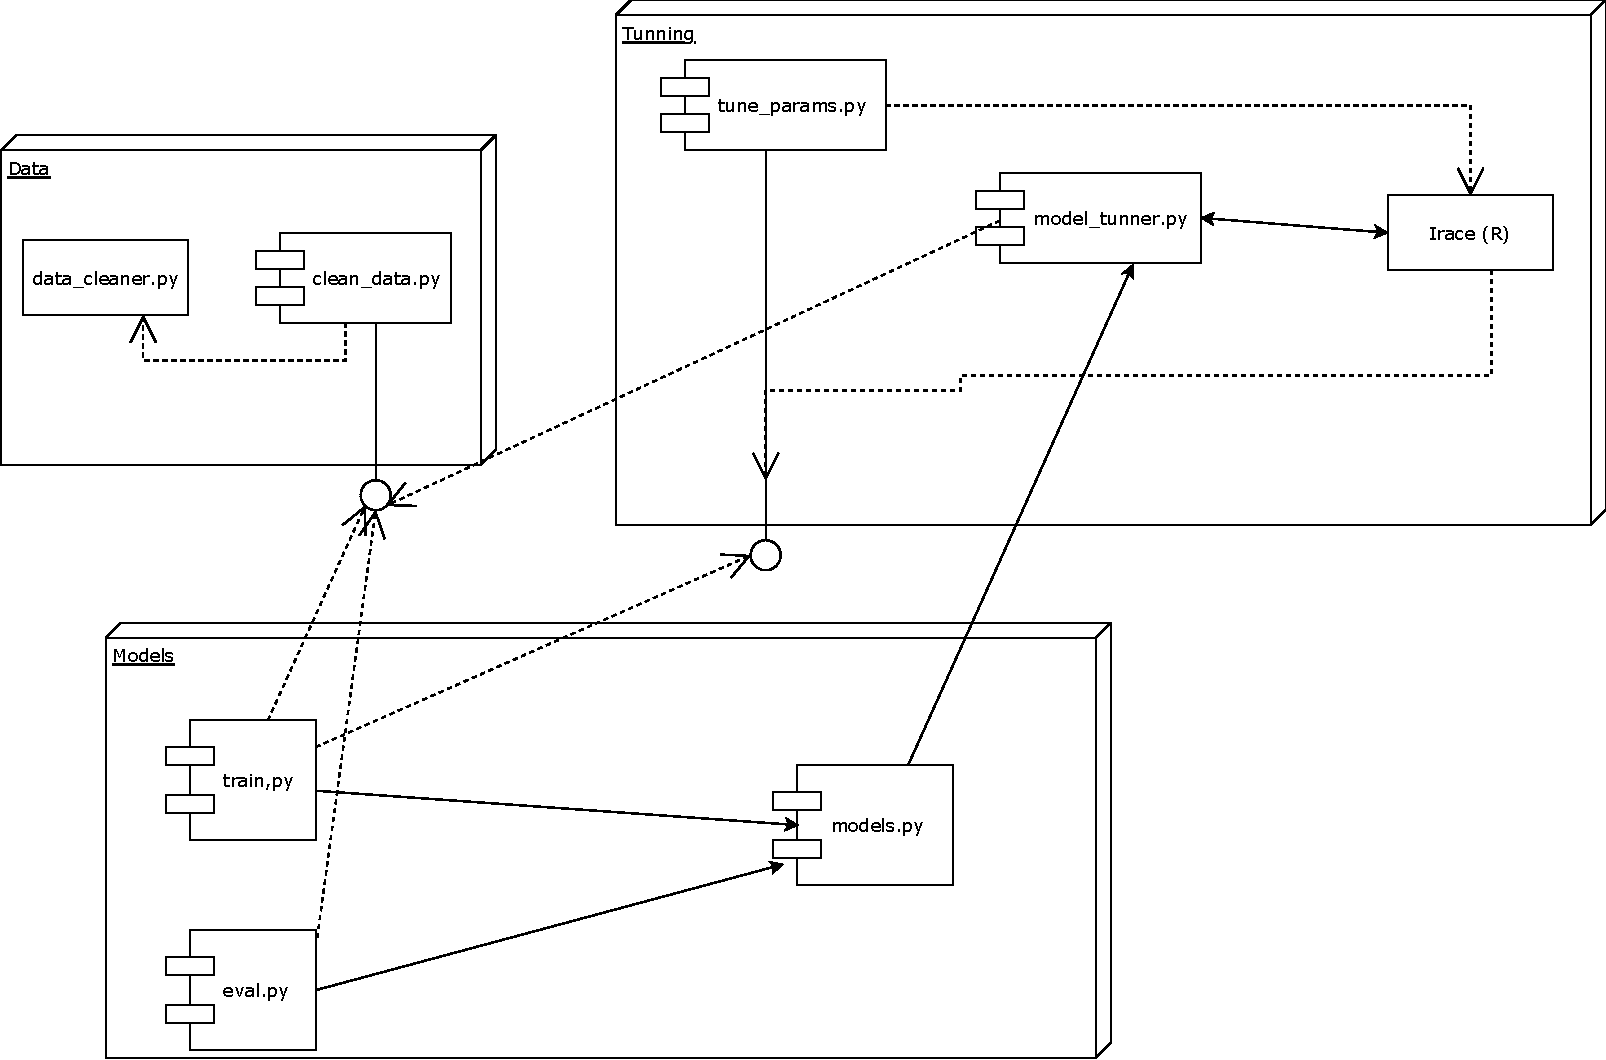
\includegraphics[width=1\textwidth]{images/sistema_modeling_mosquitos}%
          \caption{Sistema para el ajuste de parámetros y modelado}\label{fig:sistema_modelado}
          \end{figure}

        \par En el módulo \verb|data|, como se puede deducir de su nombre,
          es el encargado de limpiar los conjuntos de datos y generar los
          bloques de entrenamiento, validación y las instancias para realizar
          el ajuste de hiperparámetros de cada algoritmo.

        \par \verb|models| es el módulo dedicado a definir los algoritmos y
          posee los \textit{scripts} para el entrenamiento y
          evaluación de los mismos. Sumado a ésto, en este modulo se encuentra
          el archivo donde se deben colocar los modelos que serán utilizados
          en el modelado.

        \par \verb|tunning| es el módulo encargado del ajuste de hiperparámetros
          de los modelos. Éste realizará una búsqueda sobre el espacio de
          parámetros para encontrar los óptimos para cada algoritmo. Este
          procedimiento utiliza la herramienta \textit{irace} del lenguaje
          \textit{R} desde una interfaz de \textit{Python}.

        \par Más detalles de código se encuentran en el Anexo \ref{Anexo_codigo}.



    \subsection{Modelos lineales}

      \par Experiencias previas en aplicaciones epidemiológicas de
        modelado utilizando variables ambientales obtenidas de sensores
        remotos han reportado buenos resultados con este
        enfoque \cite{akodon_modeling, multilinear_apli, modis_data}.
        En este caso se utilizó un modelo de regresión lineal tradicional y
        una regresión \textit{Ridge}, esta última con la regularización de
        \textit{Tikhonov} y validación cruzada. Cabe destacar que la
        regresión \textit{Ridge}, en la literatura de ML, se la suele denominar
        como "decaimiento de peso" (\textit{weight decay}).

  \subsection{Modelos no-lineales}

    \par A diferencia de los modelos lineales, los no-lineales son capaces de
      capturar relaciones funcionales más complejas entre los datos, con el costo
      de una complejidad computacional más grande y una carga mucho mayor para el
      usuario que debe realizar un trabajo más fino de ajuste del modelo (la
      selección de hiperparámetros, entre otras).

    \par Tipicamente, una regresión en el ámbito del aprendizaje automático
      incluye cuatro pasos fundamentales:
      \begin{itemize}
        \item Análisis del conjunto de datos: implica extraer variables de interés, quitar redundacia y valores que generen
              ruido, etc
        \item Arquitectura: Selección del algoritmo y de los hiperparámetros como
              la cantidad de capas y neuronas en una ANN, el número de vecinos en
              el algoritmo de K-vecinos más cercanos, etc.
        \item La etapa de entrenamiento-validación: los parámetros del modelo
              se ajustan y se realizan técnicas de validación de dicho modelo para
              medir el desempeño del modelo para generalizar a nuevos datos.
        \item Utilizar el modelo con datos nuevos.
      \end{itemize}
      Estos pasos se implementaron utiliizando, mayormente, funciones disponibles
      en la librería \textit{scikit-learn} ya mencionada.

    \par La configuración o selección del conjunto óptimo de hiperparámetros
      en este tipo de modelos no-lineales es un problema complejo. Ésto
      podría realizarse a mano o utilizando herramientas semi automáticas. Lo primero
      no es buena práctica dado que podría generar un sesgo sobre los valores
      obtenidos y, además, el gran número de posibles combinaciones requeriría
      mucho tiempo del usuario en ésta tarea, aún así hay ocasiones en las
      que se utiliza esta metodología.

    \par Para realizar el ajuste de hiperparámetros, en este trabajo para la
      utilizó el paquete \textbf{\textit{IRace}}
      (\textit{Iterated Racing for Automatic Algorithm Configuration}) \cite{irace}.
      Ésta herramienta realiza un procedimiento iterativo capaz de encontrar
      automáticamente la configuración de hiperparámetros más apropiada
      dadas las instancias de datos generadas para esta etapa.
      Ésta está disponible gratuitamente para el lenguaje \textbf{R} en
      \url{http://iridia.ulb.ac.be/irace/}.

    \par Para evitar el sobre-entrenamiento (\textit{overfitting}), el ajute
      fue hecho automáticamente con datos de otras ciudades: Clorinda, Iguazú
      y Pampa.


    \subsubsection{\textit{Support Vector Regressor} (SVR)}
      \par Las \textit{Support Vector Machines} son una clase de técnica supervisada
        que construyen tanto reglas de decisiones lineales como no-lineales
        y modelos de regresión. En este caso se utilizó el algoritmo \verb|SVR|
        del módulo \verb|SVM|. Éste método implementa una regresión
        \textit{Epsilon-Support Vector}. Luego de la etapa de ajuste de
        hiperparámetros, el valor para la penalidad es de $C = 0.887453$, y
        el núcleo de función de base radial (RBF) con un valor de
        $gamma = 0.015561$.


    \subsubsection{\textit{Perceptron Multicapa} (MLP)}
      \par Las redes neuronales son contruidas a partir de una gran cantidad
        de unidades sencillas altamente conectadas entre sí. Ellas pueden
        ser entrenadas para generar aproximadores universales de funciones.
        Se utilizó la clase \verb|MLPRegressor| del módulo \verb|neural\_network|.
        Ésta clase implementa una técnica de regresión utilizando un MLP. Para
        ello optimiza el error cuadrático utilizando el \textit{LBFGS} y
        el descenso estocástico por grandiente.
        Luego de la etapa de ajuste, se obtuvo un valor para el término
        de regularización cuadrática de $alpha = 0.070921$, y un total de
        tres capas y con tres neuronas cada unas completan la arquitectura
        del modelo. La activación es hecha por la función lineal
        rectificada $f(x) = max\{0, x\}$.


    \subsubsection{Regresión de K-Vecinos Más Cercanos (KNNR)}
      \par Se utilizó la clase \verb|K-NeighborsRegressor|. Este método
        infiere una regresión basada en los k-vecinos más cercanos. El
        objetivo es predicho por una interpolación local de los objetivos
        en el entorno de vecinos del conjunto de datos de entrenamiento.
        El cojunto de datos original se descompuso utilizando componentes
        principales (\textit{PCA}), sólo cinco fueron usados. Luego de la etapa
        de ajuste, se obtuvo que el número de vecinos $n\_neighbors = 4$,
        la función de pesos utilizada en predicción que resultó generar mejor
        desempeño fue $weights = uniform$, la métrica utilizada para medir la
        distancia fue $metric = Chebyshev$ y el algoritmo que nuestro modelo
        utiliza para calcular los vecinos más cercanos resultó ser
        $algorithm = ``brute"$.

    \subsubsection{Regresión de Árboles de Decisión (DTR)}
      \par Los árboles de decisión son reglas de clasificación construidas de
      forma incremental, a partir de las cuales se puede aprender un modelo
      de regresión. En este trabajo se utilizó la clase \verb|K-NeighborsRegressor|
      del módulo \verb|tree|. Nuevamente, se utilizó \textit{PCA} pero, esta
      vez, se conservaron sólo los dos primeros componentes. Además, luego de
      dicha etapa se concluye que la regla de división sea $splitter = ``best"$,
      el valor máximo para la profundida del árbol $max_depth = 3$ y el mínimo
      valor de muestras requeridas para dividir un nodo interno es
      $min\_samples\_leaf = 5$.

      \par La elección del número de componentes en el \textit{PCA} para los
      dos últimos métodos fue basada en prueba y error, buscando por el
      subconjunto más pequeño que produzca buenos resultados.


  \section{Evaluación y análisis de los modelos generados}

    \par La Figura \ref{fig:ridge_vs_time} muestra los resultados tanto del
      modelo lineal clásico como el \textit{Ridge}. Estos resultados concuerdan
      con estudios previos. Ambos regresores lineales producen resultados muy
      similares, por lo que resulta evidente que es preferible utilizar el
      primero debido al menor costo computacional que requiere.

      \begin{figure}[hbt]
      \centering%
      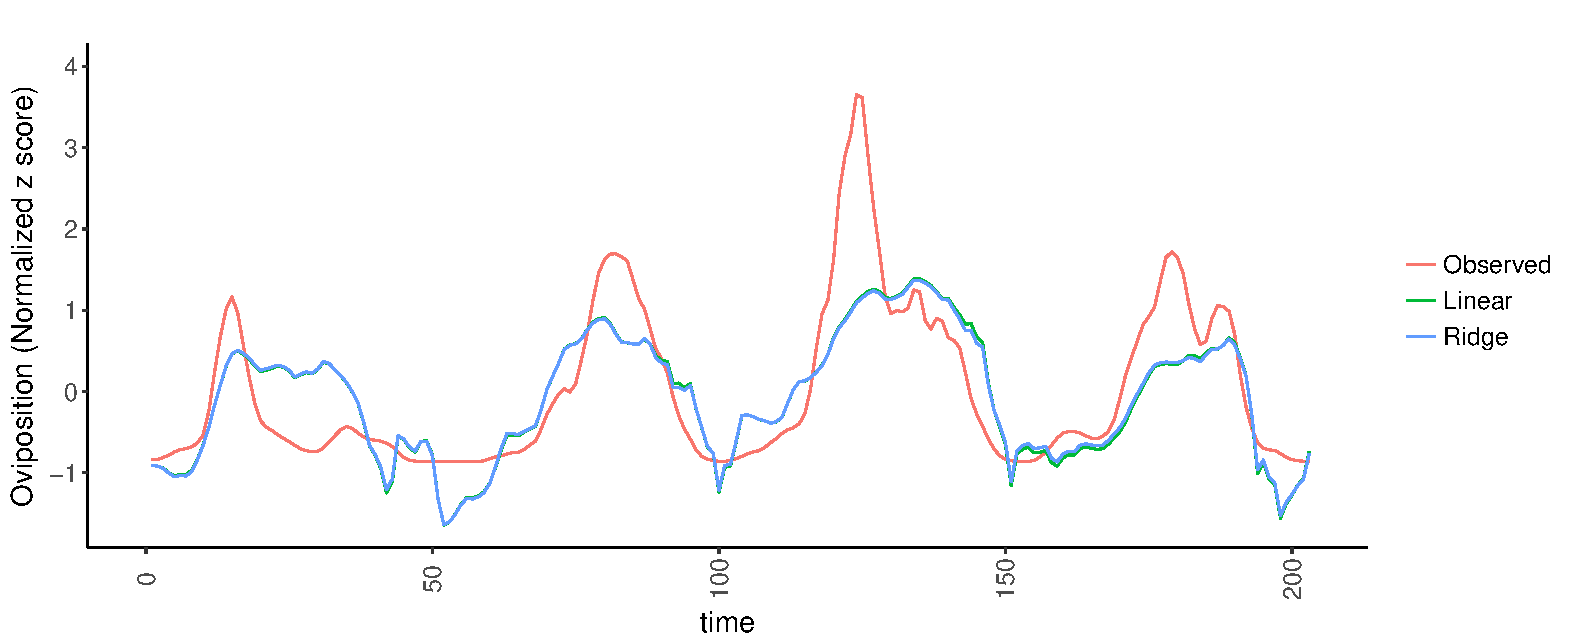
\includegraphics[width=0.9\textwidth]{images/RidgeVsTime}%
      \caption{\textit{Z-score} observado, regresiones lineales tradicional y
               \textit{Ridge}}\label{fig:ridge_vs_time}
      \end{figure}

    \par Los regresores lineales no se adecúan a los picos de los datos
    observados, y tienden a subestimar los valor más pequeños.

    \par La Figura \ref{fig:svr} muestra los datos observados y el resultado
      del procedimiento de regresión por \textit{SVR}. Este último no modela los
      picos de los primeros, pero si produce un ajuste relativamente bueno
      en la mayor parte de los datos.
      \begin{figure}[hbt]
      \centering%
      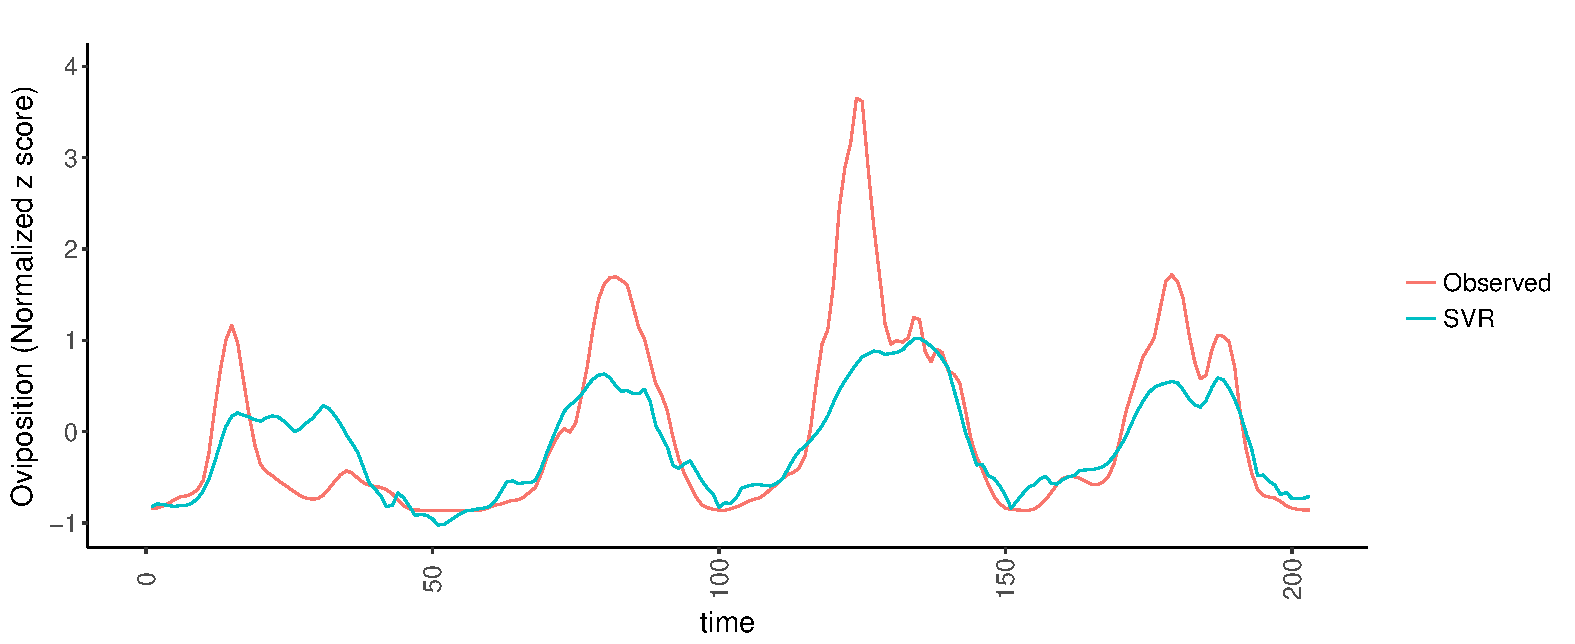
\includegraphics[width=0.9\textwidth]{images/svr}%
      \caption{\textit{Z-score} observado y regresión SVR}\label{fig:svr}
      \end{figure}


    \par La Figura \ref{fig:mlp} muestra los resultados del ajuste de
    los datos observados utilizando la técnica de \textit{MLP}. Dicho ajuste es muy
    bueno, aunque el modelo sobreestima los datos alrededor de la semana 25
    del estudio, y los subestima alrededor del último pico.
      \begin{figure}[hbt]
      \centering%
      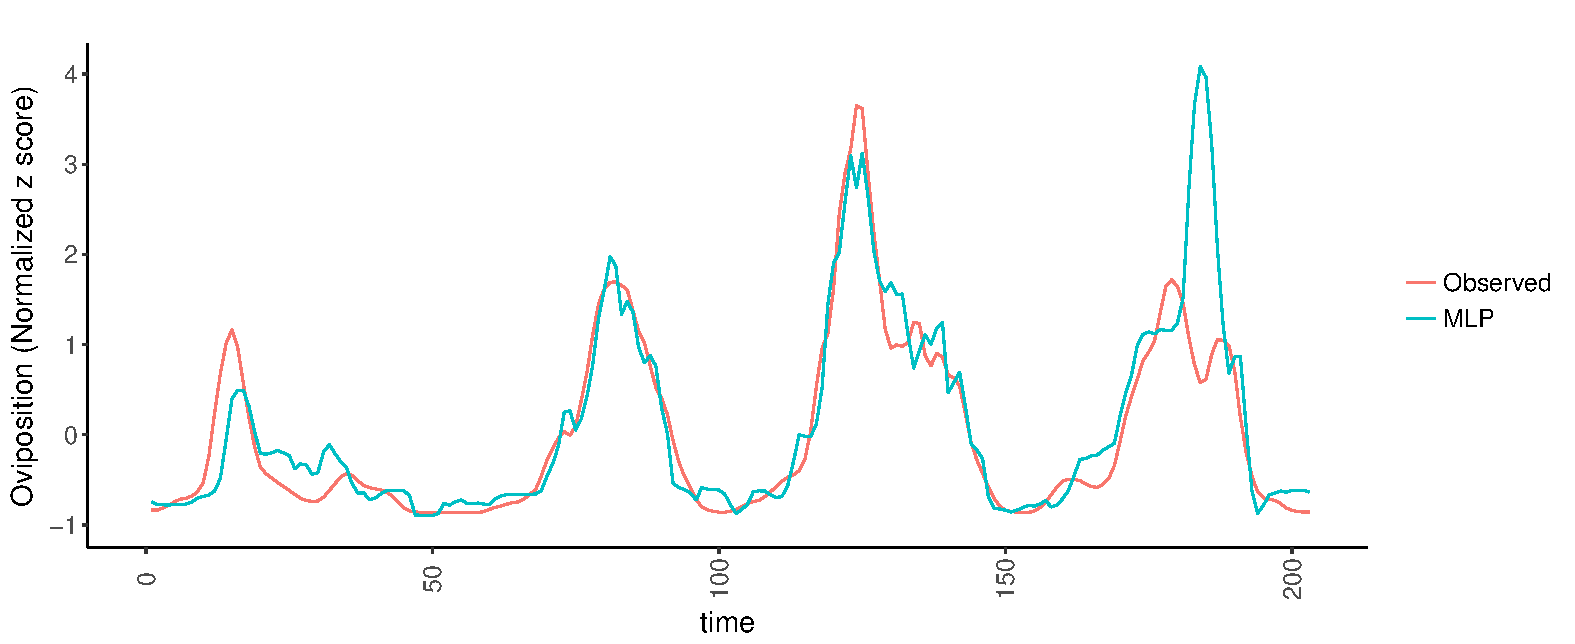
\includegraphics[width=0.9\textwidth]{images/mlp}%
      \caption{\textit{Z-score} observado y regresión MLP}\label{fig:mlp}
      \end{figure}


  \par La Figura \ref{fig:knn} muestra los resultados producidos por el procedimiento
    de \textit{KNN}. Se observa que, también, este modelo es muy bueno aunque
    falla siguiendo a los dos picos más altos. El primero, alrededor de la semana
    125 es subestimado, y el segundo, que está cerca de la semana 180, es
    sobreestimado.

    \begin{figure}[hbt]
    \centering%
    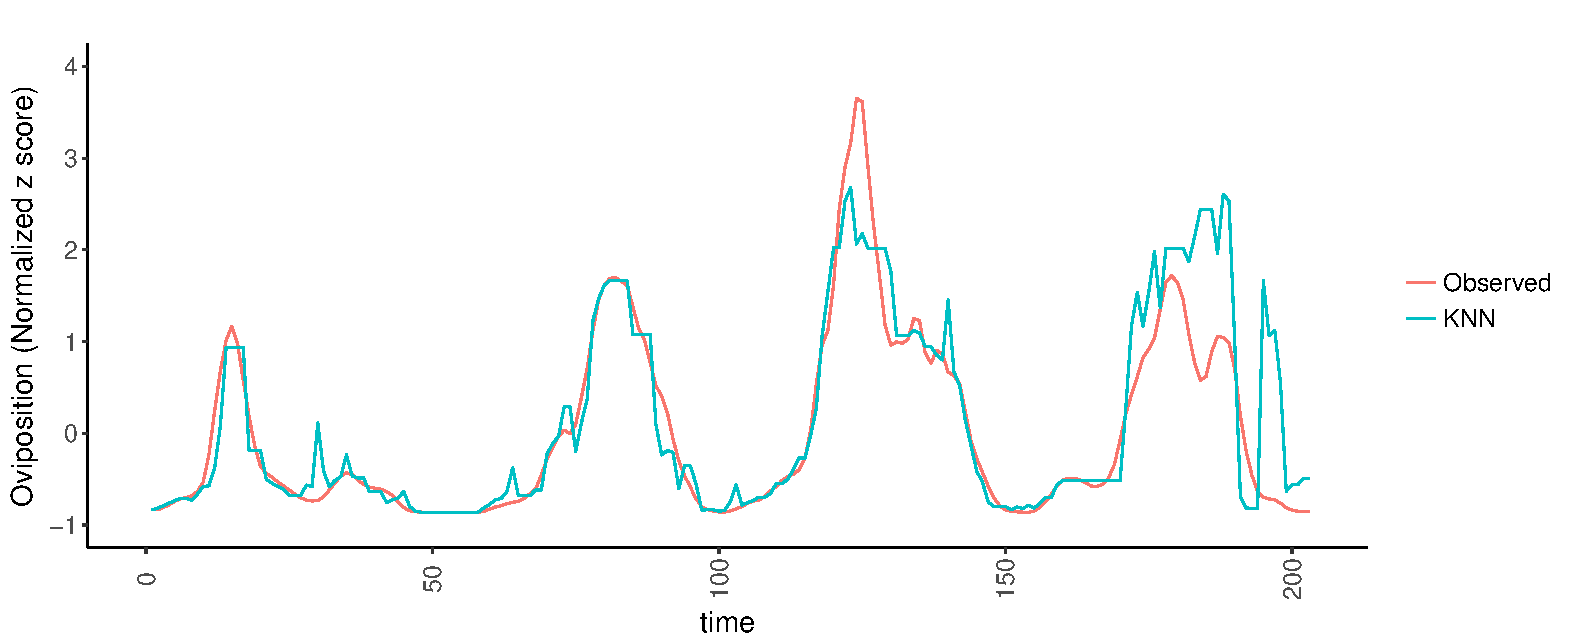
\includegraphics[width=0.9\textwidth]{images/knn}%
    \caption{\textit{Z-score} observado y regresión KNN}\label{fig:knn}
    \end{figure}


  \par La Figura \ref{fig:dtr} muestra el resultado de aplicar \textit{DTR}.
    La estructura de este procedimiento produce salidas
    planas que, sin embargo, siguen de cerca los datos observados.
    Es importante recordar que en todas las figuras anteriores, las últimas
    40 semanas no fueron utilizadas para construir los modelos, por lo que
    han sido completamente predichas.

    \begin{figure}[hbt]
    \centering%
    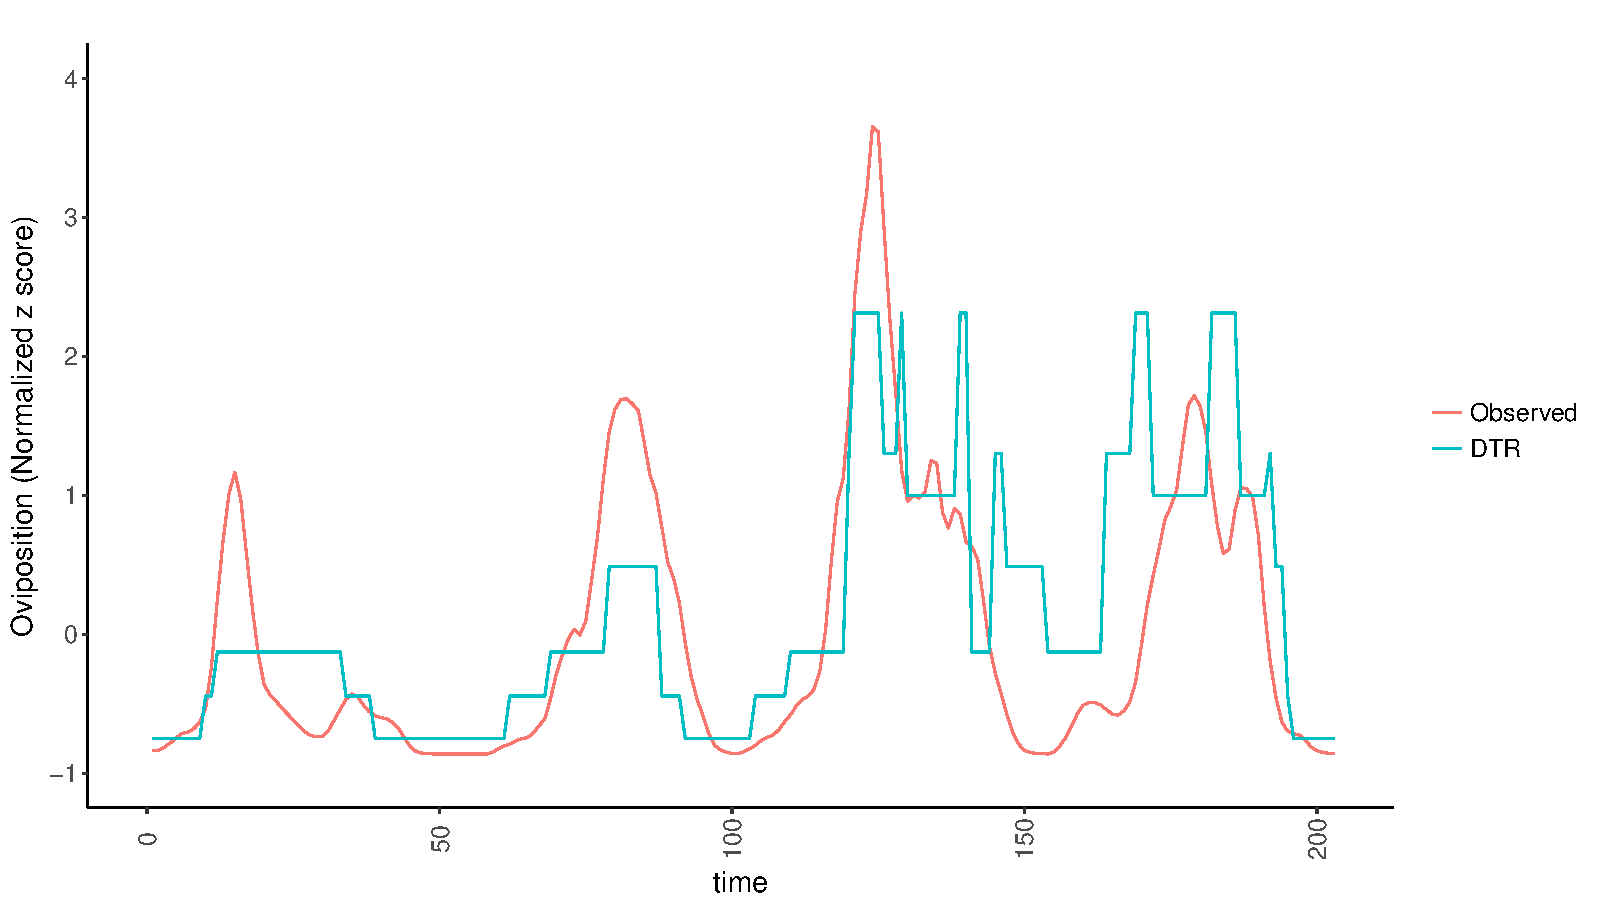
\includegraphics[width=0.9\textwidth]{images/dtr}%
    \caption{\textit{Z-score} observado y regresión DTR}\label{fig:dtr}
    \end{figure}



  \par La tabla \ref{Tab:Summary} presenta un resumen de los datos obsevados
    y los ajustados: los valores minimos (Mín) y los máximos (Máx), el
    primer ($q_{1/4}$) y tercer cuartil ($q_{3/4}$), la mediana ($q_{2/4}$)
    y la media.

  \begin{table}[hbt]
  \centering
  \caption{Resumen de los datos observados y los ajustados}\label{Tab:Summary}
  \begin{tabular}{*7{r}}
  \toprule
  &Mín	&$q_{1/4}$	&$q_{1/2}$	&Media	&$q_{3/4}$	&Máx\\ \cmidrule(lr){2-7}
  Observado	&$-0.863$	&$-0.742$	&$-0.487$	&$0.000$	&$0.704$	&$3.652$\\
  Lineal	&$-1.641$	&$-0.716$	&$ 0.027$	&$-0.087$	&$0.462$	&$1.387$\\
  Ridge	&$-1.638$	&$-0.680$	&$ 0.028$	&$-0.084$	&$0.459$	&$1.370$\\
  MLP	&$-0.894$	&$-0.677$	&$-0.323$	&$0.093$	&$0.716$	&$4.084$\\
  DTR	&$-0.752$	&$-0.752$	&$-0.128$	&$0.138$	&$0.998$	&$2.312$\\
  KNNR	&$-0.863$	&$-0.699$	&$-0.501$	&$0.099$	&$1.033$	&$2.679$\\
  SVR	&$-1.021$	&$-0.601$	&$-0.232$	&$-0.147$	&$0.309$	&$1.023$\\
  \bottomrule
  \end{tabular}
  \end{table}

  \par La Tabla \ref{Tab:Summary} revela los siguientes hechos:

    \begin{itemize}
      \item Las regresiones lineal y \textit{Ridge} exageran los minimos, ya
        que producen valores que son aproximadamente el doble que los observados.
      \item El Perceptron Multicapa exagera el máximo por alrededor de un \SI{10}{\percent},
        mientras que los otros modelos subestiman dicho valor. Notar que el \textit{SVR}
        aplana el máximo por un factor de aproximadamente 3.6.
      \item La media y mediana observadas difieren notablemente, sugiriendo que
        los modelos están significativamente sesgados a la izquierda.
      \item El valor más cercano al observado, de la mediana, es producido por
        \textit{KNN}, el cual también conduce a un valor cercado de la media.

    \end{itemize}


    \par La Figura \ref{fig:scatter} muestra los datos observados y predichos
      como un \textit{scatterplot}. Esta figura revela que ninguno de los modelos
      es capaz de seguir los valores más grandes observados, y que los modelos
      Lineal, \textit{Ridge} y \textit{SVR} son los menos aptos para esta
      tarea, mientras que \textit{MLP} es la más adecuada. Además se notó que
      este último modelo es el más propenso a sobreestimar los datos. Cabe
      destacar que la subestimación es, para el punto de vista de la aplicación,
      más peligroso que la sobreestimación, dado que el primero tiende a
      ser un falso indicador negativo que puede llevar a no disparar medidas
      de prevención en casos en que efectivamente se necesiten.
      \begin{figure}[hbt]
      \centering%
      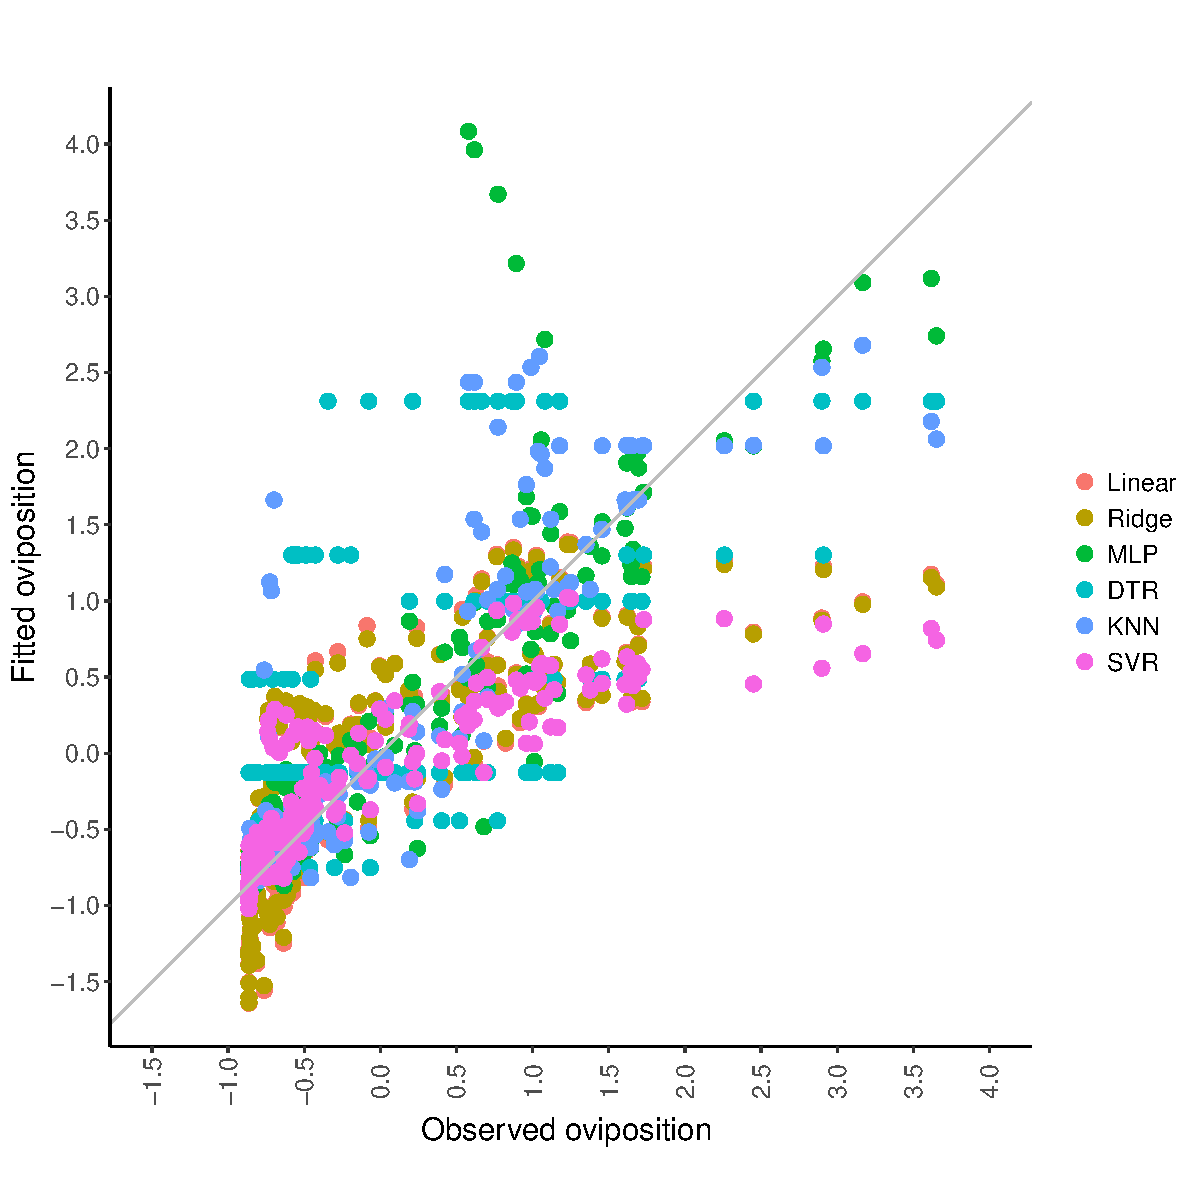
\includegraphics[width=0.6\textwidth]{images/scatterplot}%
      \caption{Scatterplot de los valores observados y predichos}\label{fig:scatter}
      \end{figure}



    \par A continuación se analizarán los errores. Las Figuras \ref{fig:Histograms}
    y \ref{fig:Boxplots} muestran, respectivamente, los histogramas y boxplots
    de los errores producidos por cada modelo. Los errores generados por
    \textit{KNN} son los más concentrados alrededor de cero, seguidos por el
    \textit{MLP}. Los dos errores más extendidos son se corresponden con
    las regresiones lineales. Éste es un indicador de que los modelos
    obotenidos utilizando simples técnicas lineales son los peores entre los
    considerados en este trabajo.
      \begin{figure}
      \centering
      \subfigure[Histogramas\label{fig:Histograms}]{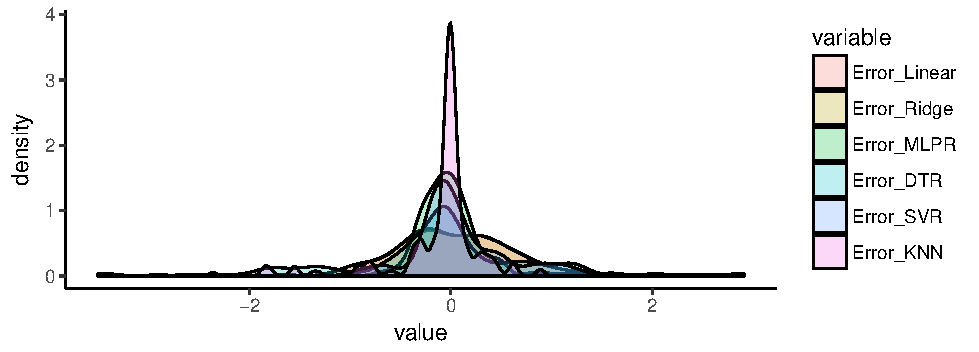
\includegraphics[width=.8\linewidth]{images/histogram_error}}
      \subfigure[Boxplots\label{fig:Boxplots}]{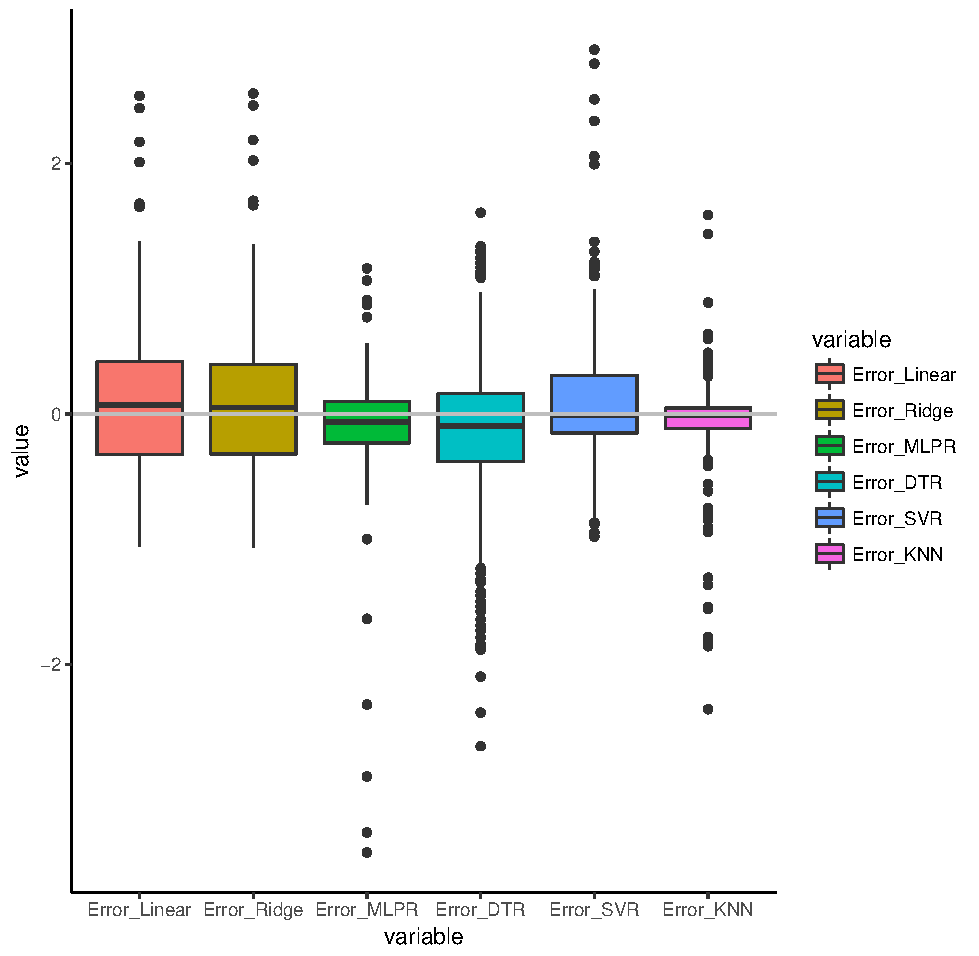
\includegraphics[width=.8\linewidth]{images/boxplot_error}}
      \caption{Errores}\label{fig:Residuals}
      \end{figure}


  \par La Tabla \ref{Tab:Quality} presenta las medidas de calidad de los modelos
  aquí considerados: los coeficientes de la correlación de \textit{Pearson}
  entre los valores observados y ajustados, usando el conjunto de datos
  completo (Corr11) y sobre el 20\% para la validación (CorrL20); además,
  el Error Cuadrático Medio sobre el conjunto de datos completo (MSE), y
  sólo sobre los datos de validación (MSEL20). Siguiendo \cite{dynamics_of_dengue},
  también se incluyó el \textit{z-score} medio obtenido de la validación
  cruzada y su desviación estándar (SD del Z-Score).


  \begin{table}[hbt]
  \centering
  \caption{Medidas de calidad de los modelos}\label{Tab:Quality}
  \begin{tabular}{*7{r}}
  \toprule
  & Corr11
  & MSE
  & Z-Score Medio
  & SD del Z-Score
  & CorrL20
  & MSEL20 \\ \midrule
  Lineal
  &$0.774$
  &$0.624$
  &$1.108$%&\boldmath$1.108$  %CARO: cambio
  &$0.278$
  &$0.890$
  &$0.580$\\
  Ridge
  &$0.775$
  &$0.621$
  &$1.072$
  &$0.277$
  &$0.896$
  &$0.566$ \\
  SVR
  &$0.837$
  &$0.613$
  &\boldmath$0.834$   %CARO: cambio
  &$0.490$
  &\boldmath$0.967$
  &\boldmath$0.464$ \\
  MLP
  &$0.875$
  &$0.528$
  &$1.086$
  &$0.288$
  &$0.727$
  &$1.023$ \\
  KNN
  &\boldmath$0.888$
  &\boldmath$0.494$
  &$0.981$
  &$0.362$
  &$0.797$
  &$0.936$\\
  DTR
  &$0.679$
  &$0.768$
  &$1.148$
  &$0.544$
  &$0.532$
  &$1.131$ \\
  \bottomrule
  \end{tabular}
  \end{table}

  \section{Discusión de resultados obtenidos en la primer etapa}

    \par Un punto interesante que aparece en los resultados es que todos los
      modelos aquí presentados ajustan bien en los patrones principales
      pero no necesariamente en los picos extremos. Una hipótesis es que la población
      del vector se desconecta de las variables macroambientales/climáticas
      cuando las condiciones son óptimas y, nuevamente, se restringe cuando las
      condiciones ambientales son suboptimas. De hecho, es razonable el hecho de
      que no podemos esperar ajustar exactamente la población urbana del vector
      sólo basándonos en variables macroambientales a gran escala.


    \par Teniendo en cuenta la bondad de ajuste incluida en las Tablas
      \ref{Tab:Summary} y \ref{Tab:Quality}, y un análisis de errores, podríamos
      considerar que \textit{KNN} aparenta ser el mejor método para este problema.
      Tiene una correlación cercana al 90\%, considerablemente mayor al
      75\%, el valor típico obtenido por las técnicas lineales.

  \par El valor medio del \textit{z-score} llevaría a elegir el \textit{SVR}
    como la mejor técnica \cite{ml_rainfall}. Cabe destacar que la desviación
    estándar de esta medición de calidad es tan alta que es poco probable que
    sea una buena elección en sí misma. Por esta razón, si seguimos un
    enfoque holístico en las próximas conclusiones.


  \par Si tenemos en cuenta las seis métricas de la Tabla \ref{Tab:Quality},
    es clara la conclusión de que los mejores métodos para modelar la población
    del vector basada en variables ambientales derivadas de información satelital
    son: \textit{K-vecinos más cercanos}, \textit{Perceptron
    Multicapa} y \textit{Support Vector Machine}.


\section{Problemáticas de un sistema regional de modelado de poblaciones de mosquito}

  \par La tarea de modelar la población de mosquitos a nivel regional
    trae consigo numerosas problemáticas, algunas de las cuales ya fueron
    mencionadas en la sección de Motivación y Marco Teórico.

  \par En este trabajo, un problema que encontramos es la escases de datos de campo que existen:
    el desempeño de estos algoritmos se podría mejorar sustancialmente utilizando
    conjuntos de datos más grandes.
    Aunque el período utilizado es grande en comparación con trabajos similares
    sobre la población vectorial, dicho conjunto sigue siendo
    muy pequeño desde el punto de vista del aprendizaje automático.

  \par Otro problema, no menos importante teniendo en cuenta el objetivo final
    de los esfuerzos puestos en este sentido (tener modelos operativos de
    riesgo), es la gran escases de puntos (ciudades) de los cuales se posee información
    de campo (oviposición). Esto resulta un problema dado que si los modelos son
    entrenados con datos de un punto geográfico \textbf{A} (Tartagal, por ejemplo), a
    priori no podemos asegurar que serán capaces de ajustar correctamente al
    comportamiento de la variable objetivo de un punto \textbf{B} (Córdoba, por ejemplo).
    Pues ni siquiera se poseen datos para validar dicha conducta.
    Esto limita el alcance regional de las herramientas de este tipo.

%\end{document}
